% SourceSink User Manual
% Build with:  ./build.sh   (Tectonic or XeLaTeX via latexmk)
\documentclass[11pt,oneside]{book}

% ---------------------------------------------------------------- packages
\usepackage[letterpaper,margin=1in,headheight=14pt]{geometry}
\usepackage{fontspec}
\usepackage{unicode-math}
% Fonts are named by file so the build works with Tectonic and TeX Live alike.
\setmainfont{texgyrepagella}[Extension=.otf,UprightFont=*-regular,BoldFont=*-bold,
  ItalicFont=*-italic,BoldItalicFont=*-bolditalic]
\setsansfont{texgyreheros}[Extension=.otf,UprightFont=*-regular,BoldFont=*-bold,
  ItalicFont=*-italic,BoldItalicFont=*-bolditalic,Scale=0.92]
\setmonofont{lmmono10}[Extension=.otf,UprightFont=*-regular,Scale=0.95]
\setmathfont{texgyrepagella-math.otf}
\usepackage{microtype}
\usepackage{amsmath}
\usepackage{graphicx}
\usepackage{booktabs}
\usepackage{tabularx}
\usepackage{longtable}
\usepackage{array}
\usepackage{enumitem}
\usepackage{xcolor}
\usepackage[most]{tcolorbox}
\usepackage{listings}
\usepackage{titlesec}
\usepackage{fancyhdr}
\usepackage{caption}
\usepackage{tikz}
\usepackage[hidelinks]{hyperref}
\usepackage{bookmark}

% ---------------------------------------------------------------- colours
\definecolor{accent}{HTML}{5868E8}
\definecolor{accentsoft}{HTML}{E7E9FD}
\definecolor{ink}{HTML}{111827}
\definecolor{muted}{HTML}{5F6776}
\definecolor{stockband}{HTML}{DFE5FD}
\definecolor{flowband}{HTML}{D3F3DE}
\definecolor{convband}{HTML}{EBE1FC}
\definecolor{notebg}{HTML}{F7F8FA}
\definecolor{warnbg}{HTML}{FFF4E5}
\definecolor{warnline}{HTML}{E8A33D}
\definecolor{codebg}{HTML}{F4F5F8}

\hypersetup{colorlinks=true,linkcolor=accent,urlcolor=accent,citecolor=accent,
  pdftitle={SourceSink User Manual},pdfauthor={SourceSink contributors}}

% ---------------------------------------------------------------- headings
\titleformat{\chapter}[display]
  {\normalfont\sffamily\color{ink}}
  {\color{accent}\large\bfseries\MakeUppercase{\chaptertitlename}\ \thechapter}
  {6pt}
  {\Huge\bfseries}
  [\vspace{4pt}{\color{accent}\titlerule[1.2pt]}]
\titlespacing*{\chapter}{0pt}{0pt}{24pt}
\titleformat{\section}{\normalfont\sffamily\Large\bfseries\color{ink}}{\color{accent}\thesection}{0.8em}{}
\titleformat{\subsection}{\normalfont\sffamily\large\bfseries\color{ink}}{\color{accent}\thesubsection}{0.8em}{}
\titleformat{\subsubsection}{\normalfont\sffamily\normalsize\bfseries\color{ink}}{}{0em}{}

\pagestyle{fancy}
\fancyhf{}
\fancyhead[L]{\sffamily\small\color{muted}SourceSink User Manual}
\fancyhead[R]{\sffamily\small\color{muted}\nouppercase{\leftmark}}
\fancyfoot[C]{\sffamily\small\color{muted}\thepage}
\renewcommand{\headrulewidth}{0.4pt}
\renewcommand{\headrule}{{\color{accentsoft}\hrule width\headwidth height\headrulewidth}}
\fancypagestyle{plain}{\fancyhf{}\fancyfoot[C]{\sffamily\small\color{muted}\thepage}\renewcommand{\headrulewidth}{0pt}}

\captionsetup{font={small,sf},labelfont={bf,color=accent},margin=10pt}
\setlist{itemsep=2pt,topsep=4pt}
\setlength{\parskip}{4pt}
\renewcommand{\topfraction}{0.9}
\renewcommand{\bottomfraction}{0.8}
\renewcommand{\textfraction}{0.08}
\renewcommand{\floatpagefraction}{0.75}
\setcounter{topnumber}{3}
\setcounter{totalnumber}{4}
\renewcommand{\bibname}{References}

% ---------------------------------------------------------------- boxes
\newtcolorbox{tryit}[1][]{enhanced,breakable,before skip=10pt,after skip=10pt,colback=accentsoft!55,colframe=accent,
  boxrule=0pt,leftrule=3pt,arc=2pt,left=10pt,right=10pt,top=6pt,bottom=6pt,
  fonttitle=\sffamily\bfseries\color{accent},coltitle=accent,colbacktitle=accentsoft!55,
  title={#1},attach title to upper={\par\smallskip}}
\newtcolorbox{note}[1][Note]{enhanced,before skip=10pt,after skip=10pt,colback=notebg,colframe=muted!40,
  boxrule=0pt,leftrule=3pt,arc=2pt,left=10pt,right=10pt,top=6pt,bottom=6pt,
  fonttitle=\sffamily\bfseries\color{muted},coltitle=muted,colbacktitle=notebg,
  title={#1},attach title to upper={\par\smallskip}}
\newtcolorbox{caution}[1][Watch out]{enhanced,before skip=10pt,after skip=10pt,colback=warnbg,colframe=warnline,
  boxrule=0pt,leftrule=3pt,arc=2pt,left=10pt,right=10pt,top=6pt,bottom=6pt,
  fonttitle=\sffamily\bfseries\color{warnline!80!black},coltitle=warnline!80!black,colbacktitle=warnbg,
  title={#1},attach title to upper={\par\smallskip}}
\newtcolorbox{mathbox}[1][The mathematics]{enhanced,breakable,before skip=12pt,after skip=12pt,colback=white,colframe=accent!35,
  boxrule=0.6pt,arc=3pt,left=12pt,right=12pt,top=8pt,bottom=8pt,
  fonttitle=\sffamily\bfseries\small\color{white},colbacktitle=accent!85,title={#1}}

% numbered steps
\newlist{steps}{enumerate}{1}
\setlist[steps]{label={\sffamily\bfseries\color{accent}\arabic*},leftmargin=2em,itemsep=4pt}

% ---------------------------------------------------------------- code
\lstdefinestyle{cli}{basicstyle=\ttfamily\small,backgroundcolor=\color{codebg},
  frame=single,framerule=0pt,framesep=6pt,xleftmargin=6pt,xrightmargin=6pt,
  columns=fullflexible,keepspaces=true,breaklines=true,showstringspaces=false,
  aboveskip=8pt,belowskip=8pt,commentstyle=\color{muted},
  literate={−}{{-}}1 {→}{{$\rightarrow$}}1 {·}{{$\cdot$}}1 {±}{{$\pm$}}1 {²}{{$^2$}}1 {₂}{{$_2$}}1}
\lstset{style=cli}

% ---------------------------------------------------------------- helpers
\newcommand{\ui}[1]{\textsf{\textbf{#1}}}                       % a button or label
\newcommand{\key}[1]{\tikz[baseline=(k.base)]\node[draw=muted!60,fill=notebg,rounded corners=2pt,inner sep=2pt,font=\sffamily\small](k){#1};}
\newcommand{\el}[1]{\texttt{#1}}                                % a model element
\newcommand{\shot}[3][\textwidth]{\begin{figure}[htbp]\centering
  \includegraphics[width=#1]{img/#2}\caption{#3}\label{fig:#2}\end{figure}}
\newcommand{\stockchip}{\tikz[baseline=-0.6ex]\node[fill=stockband,rounded corners=2pt,inner sep=2pt,font=\sffamily\scriptsize]{stock};}
\newcommand{\flowchip}{\tikz[baseline=-0.6ex]\node[fill=flowband,rounded corners=2pt,inner sep=2pt,font=\sffamily\scriptsize]{flow};}
\newcommand{\convchip}{\tikz[baseline=-0.6ex]\node[fill=convband,rounded corners=2pt,inner sep=2pt,font=\sffamily\scriptsize]{converter};}

\begin{document}

% ================================================================ title page
\begin{titlepage}
\begin{tikzpicture}[remember picture,overlay]
  \fill[accent] (current page.north west) rectangle ([yshift=-9.2cm]current page.north east);
  \fill[accent!80!black] ([yshift=-9.2cm]current page.north west) rectangle ([yshift=-9.45cm]current page.north east);
  % a small stock-and-flow mark
  \begin{scope}[shift={([xshift=-5.6cm,yshift=-3.0cm]current page.north east)},scale=0.9]
    \draw[white,line width=2.4pt,-{latex}] (-2.6,0) -- (-0.75,0);
    \draw[white,line width=2.4pt] (0.75,0) -- (2.2,0);
    \draw[white,line width=2.4pt,-{latex}] (2.2,0) -- (3.0,0);
    \fill[white,rounded corners=4pt] (-0.75,-0.55) rectangle (0.75,0.55);
    \fill[accent!35,rounded corners=4pt] (-0.75,0.15) rectangle (0.75,0.55);
    \fill[white] (-1.95,0.25) -- (-1.55,0) -- (-1.95,-0.25) -- cycle;
    \fill[white] (-1.15,0.25) -- (-1.55,0) -- (-1.15,-0.25) -- cycle;
  \end{scope}
\end{tikzpicture}
\vspace*{1.2cm}
{\sffamily\color{white}
{\fontsize{44}{48}\selectfont\bfseries SourceSink}\\[10pt]
{\LARGE User Manual}\\[6pt]
{\large Building, running and analyzing stock-and-flow models}}

\vspace{7.2cm}
{\sffamily\color{ink}
\begin{minipage}{0.62\textwidth}
\large This manual teaches system dynamics modeling with SourceSink through
worked tutorials: building a model from scratch, exploring the example
library, calibrating a model to field data, sensitivity and uncertainty
analysis, and building models in conversation with the modeling assistant.
\end{minipage}}

\vfill
{\sffamily\color{muted}
Version 0.2 \hfill October 2026\\
\url{https://github.com/anonymousacademe/sourcesink}}
\end{titlepage}

\frontmatter
\tableofcontents

% ================================================================ how to read
\chapter*{How to use this manual}
\addcontentsline{toc}{chapter}{How to use this manual}

If you are new to system dynamics, read Chapter~\ref{ch:intro} and then work
through Tutorial~1 (Chapter~\ref{ch:t1}) with the app open beside you. It
takes about twenty minutes and touches every basic tool. The other tutorials
can be done in any order; each starts from a model that ships with
SourceSink, so you never need to finish one tutorial to start another.

\begin{note}[Conventions]
Buttons and labels you click appear as \ui{Run} or \ui{Add parameter}. Keys
appear as \key{S} or \key{Ctrl}+\key{Enter}. Model element names appear in
code type, such as \el{P\_mass}. Boxes like this one hold notes; blue boxes
hold the steps of a tutorial; white boxes with a blue title hold the
mathematics behind a feature. You can skip the mathematics on a first
reading and still use every feature.
\end{note}

Chapter~\ref{ch:ref} is a reference for the editor, and the appendices
collect the equation functions, unit syntax and keyboard shortcuts. A
separate guide for AI agents and scripts, \texttt{docs/llm/cli-guide.md},
documents the command line and the MCP server in full.

\mainmatter

% ================================================================ chapter 1
\chapter{Introduction}\label{ch:intro}

\section{What SourceSink is}

SourceSink is a free, open-source tool for system dynamics: the practice of
describing a system as quantities that accumulate (\emph{stocks}) and the
rates that change them (\emph{flows}), wiring them together with the rules
that connect them (\emph{converters} and \emph{connectors}), and then
simulating forward in time to see what the structure does. Phosphorus in a
lake, adopters of a new technology, carbon in the atmosphere, fish in a
fishery and work in a project all fit this pattern.

SourceSink runs as a desktop application on Linux, Windows and macOS, in a
web browser, and from the command line. Besides drawing and running models,
it can fit a model to observations, rank which parameters matter, show the
range of outcomes under uncertainty, check units, describe a model in plain
language, and build a model with you through a conversation with an AI
assistant. It also opens legacy \texttt{.stm} and \texttt{.itm} model files.

\section{Stocks and flows in one equation}

Every stock-and-flow model rests on one idea. A stock $S$ changes only through
the flows attached to it:
\begin{mathbox}[Accumulation]
\begin{equation}
  \frac{dS}{dt} \;=\; \sum_{i} \text{inflow}_i(t) \;-\; \sum_{j} \text{outflow}_j(t),
  \qquad
  S(t) \;=\; S(t_0) + \int_{t_0}^{t} \Bigl(\sum_i \text{inflow}_i - \sum_j \text{outflow}_j\Bigr)\,d\tau .
  \label{eq:accumulation}
\end{equation}
Flows and converters are ordinary functions of the stocks, of time and of
constants. The diagram is a picture of these equations: a pipe into a stock
is a $+$ term, a pipe out of it is a $-$ term, and a dashed connector into a
flow or converter means ``this equation reads that value.''
\end{mathbox}

SourceSink solves equation~\eqref{eq:accumulation} numerically. With a time
step $\Delta t$ (called \emph{DT}), Euler's method updates each stock as
\begin{equation}
  S_{n+1} = S_n + \Delta t \Bigl(\sum_i \text{inflow}_i(t_n) - \sum_j \text{outflow}_j(t_n)\Bigr),
  \label{eq:euler}
\end{equation}
which is simple and transparent but needs a small DT for accurate results.
Section~\ref{sec:methods} describes the higher-order methods (Runge--Kutta 2
and 4, and an adaptive Runge--Kutta 4/5 called \ui{Adaptive (RK45)}) for
models that change quickly.

\section{The building blocks}

\begin{center}
\renewcommand{\arraystretch}{1.25}
\begin{tabularx}{\textwidth}{@{}l X X@{}}
\toprule
\textbf{\sffamily Element} & \textbf{\sffamily What it represents} & \textbf{\sffamily How it looks}\\
\midrule
\stockchip & A quantity that accumulates: water, people, money, phosphorus. Its equation is its \emph{initial value}. & A white card with a blue name band and its latest value.\\
\flowchip & A rate that fills or drains a stock: kg/year, people/day. & A small chip with a bow-tie mark sitting on a gray pipe.\\
\convchip & A constant or a calculation from other values. & A lavender pill; constants show their value.\\
connector & An information link: ``this equation uses that value.'' & A dashed gray arrow.\\
cloud & The outside of the model: where a flow comes from or goes to when no stock is attached. & A faint cloud at the end of a pipe.\\
\bottomrule
\end{tabularx}
\end{center}

\section{Installing SourceSink}

You do not need to compile anything. Each release on the project's Releases
page (\url{https://github.com/anonymousacademe/sourcesink/releases}) has
installers:

\begin{center}
\renewcommand{\arraystretch}{1.2}
\begin{tabularx}{\textwidth}{@{}l l X@{}}
\toprule
\textbf{\sffamily System} & \textbf{\sffamily File} & \textbf{\sffamily Notes}\\
\midrule
Any Linux & one command (below) & Installs for your user only; no root needed.\\
Debian, Ubuntu & \texttt{SourceSink-…-amd64.deb} & \texttt{sudo apt install ./SourceSink-…-amd64.deb}\\
Arch, Omarchy & \texttt{SourceSink-…-x64.pacman} & \texttt{sudo pacman -U SourceSink-…-x64.pacman}\\
Windows & \texttt{SourceSink-…-x64.exe} & The installer is not yet signed; choose \ui{Run anyway}.\\
macOS & \texttt{SourceSink-…-arm64.dmg} & Not yet signed: right-click the app and choose \ui{Open} the first time.\\
\bottomrule
\end{tabularx}
\end{center}

On Linux, this command downloads the latest release and adds SourceSink to
your application launcher:
\begin{lstlisting}
curl -fsSL https://raw.githubusercontent.com/anonymousacademe/sourcesink/main/scripts/install.sh | sh
\end{lstlisting}

To run the newest code instead, install Node.js 22.19 or newer and run
\texttt{npm install} and then \texttt{npm start} (browser) or
\texttt{npm run desktop} (desktop window) in a copy of the repository.

\section{A tour of the window}

\shot{overview.png}{The SourceSink window with the Streeter--Phelps oxygen-sag example open and run. The toolbar is at the top, the tool palette floats on the left, the diagram fills the middle, the inspector on the right shows the selected stock, and the results drawer at the bottom plots the run.}

Figure~\ref{fig:overview.png} shows the main areas:
\begin{description}[style=nextline,leftmargin=1.2em,font=\sffamily\bfseries\color{ink}]
  \item[Toolbar] \ui{New}, \ui{Open}, \ui{Save}, the example gallery
  (\ui{Examples}), the \ui{Assistant}, \ui{Describe} (a plain-language
  description of the model), \ui{Analyze} (calibration, sensitivity and
  uncertainty), undo and redo, \ui{Run}, and the light/dark theme switch.
  \item[Tool palette] Select (\key{V}), Stock (\key{S}), Flow (\key{F}),
  Converter (\key{C}), Connector (\key{K}), and \ui{Tidy up} (\key{L}), which
  re-arranges the diagram.
  \item[Canvas] The diagram. Drag to move elements, scroll to zoom, and use
  the zoom pill at the bottom left to fit the model to the window.
  \item[Inspector] The properties of whatever is selected: name, equation,
  units, documentation and element-specific options. With nothing selected
  it shows the model's run settings and scenarios.
  \item[Results drawer] Graph and table of the last run. Click a series name
  to show or hide it; \ui{Export CSV} saves the numbers.
\end{description}

% ================================================================ tutorial 1
\chapter{Tutorial 1: Build your first model}\label{ch:t1}

In this tutorial you build a model of phosphorus in a lake from nothing. It is
a classic environmental box model: a watershed delivers phosphorus to a
lake, and the lake loses it two ways, by flushing out with the outflowing
river and by settling into the sediment. You will learn to add each kind of
element, write equations with units, run the model, read the results, and
check the answer against the mathematics.

\begin{mathbox}[The lake as a box model]
Let $M$ be the phosphorus mass in the lake (kg), $L$ the external load
(kg/year), $\rho$ the flushing rate and $\sigma$ the settling rate (both per
year). Then
\begin{equation}
  \frac{dM}{dt} \;=\; \underbrace{L}_{\text{loading}}
  \;-\; \underbrace{\rho M}_{\text{flushing}}
  \;-\; \underbrace{\sigma M}_{\text{settling}} .
  \label{eq:lake}
\end{equation}
Starting from $M(0)=0$, the exact solution is
\begin{equation}
  M(t) = M^{*}\bigl(1 - e^{-t/\tau}\bigr),
  \qquad M^{*} = \frac{L}{\rho + \sigma},
  \qquad \tau = \frac{1}{\rho + \sigma}.
  \label{eq:lake-solution}
\end{equation}
With $L = 1000$~kg/year and $\rho = \sigma = 0.5$/year, the lake approaches
$M^{*} = 1000$~kg with a response time $\tau = 1$~year. For a lake volume
$V = 10^{7}$~m$^3$ the steady concentration is
$C^{*} = M^{*}/V = 10^{-4}$~kg/m$^3$ $= 0.1$~g/m$^3$ $= 100$~µg/L, the
classic result of Vollenweider's loading concept \cite{vollenweider1975}.
\end{mathbox}

\section{Add the stock}

\begin{tryit}[Step by step]
\begin{steps}
  \item Click \ui{New} in the toolbar. The canvas is empty and shows a short
  hint (Figure~\ref{fig:empty.png}).
  \item Press \key{S} (or click the stock tool in the palette), then click on
  the canvas. A stock appears and the inspector shows its properties.
  \item In the inspector, set \ui{Name} to \el{P\_mass}, \ui{Initial value}
  to \el{0}, \ui{Units} to \el{kg}, and \ui{Documentation} to
  ``Phosphorus dissolved in the lake.''
\end{steps}
\end{tryit}

\shot{empty.png}{A new, empty model. The hint in the middle reminds you of the drawing keys.}

\shot{t1-a.png}{The stock \el{P\_mass} after setting its name, initial value, units and documentation. A stock's equation is its \emph{initial value}.}

\begin{note}[Names]
Names may contain letters, digits and underscores. Spaces are converted to
underscores in equations, so \el{P mass} and \el{P\_mass} refer to the same
element. Short, readable names (\el{settling\_rate}, not \el{sr}) make the
model and its description easier to follow.
\end{note}

\section{Add the flows}

A flow is drawn by dragging. Dragging from empty canvas \emph{into} a stock
creates an inflow from a cloud; dragging \emph{out of} a stock to empty
canvas creates an outflow to a cloud; dragging from one stock to another
creates a flow between them.

\begin{tryit}[Step by step]
\begin{steps}
  \item Press \key{F}. Drag from empty canvas on the left into \el{P\_mass}.
  Name the new flow \el{loading}, set its equation to \el{1000} and its units
  to \el{kg/year}.
  \item Drag from \el{P\_mass} to empty canvas on the right. Name it
  \el{flushing}, units \el{kg/year}. Leave its equation for now.
  \item Drag from \el{P\_mass} downward to make a second outflow,
  \el{settling}, units \el{kg/year}.
\end{steps}
\end{tryit}

\shot{t1-b.png}{The stock with one inflow and two outflows. Each flow ends in a cloud: the watershed, the river downstream and the sediment are outside the model.}

\section{Add converters and connectors}

The two outflows depend on rates. Converters hold those rates, and connectors
tell each flow which values its equation may read.

\begin{tryit}[Step by step]
\begin{steps}
  \item Press \key{C} and click near \el{flushing}. Name the converter
  \el{flushing\_rate}, equation \el{0.5}, units \el{1/year}. Add a second
  converter \el{settling\_rate} the same way.
  \item Press \key{K} and drag from \el{flushing\_rate} to \el{flushing},
  then from \el{P\_mass} to \el{flushing}. Do the same for
  \el{settling\_rate} and \el{P\_mass} into \el{settling}.
  \item Select \el{flushing} and set its equation to
  \el{flushing\_rate * P\_mass}; set \el{settling} to
  \el{settling\_rate * P\_mass}. As you type, the inspector suggests names
  and functions; press \key{Tab} or \key{Enter} to accept one.
  \item Add a converter \el{volume} (\el{1e7}, units \el{m3}) and a converter
  \el{concentration} with equation \el{P\_mass / volume * 1000} and units
  \el{g/m3}, with connectors from \el{P\_mass} and \el{volume}.
\end{steps}
\end{tryit}

\shot{t1-c.png}{The finished lake model with the \el{concentration} converter selected. The factor 1000 converts kg/m$^3$ to g/m$^3$.}

\begin{note}[Why connectors matter]
An equation should only use values that are connected to it. If you type a
name that has no connector, the inspector says ``Uses \el{P\_mass} but it
isn't connected'' and offers a \ui{Connect} button that draws the connector
for you. This keeps the diagram an honest picture of the equations.
\end{note}

\section{Check the units}

SourceSink checks units as you work. A flow must be in the units of its stock
per unit of model time, and both sides of a $+$ or $-$ must agree. If you had
typed \el{kg} instead of \el{kg/year} for \el{flushing}, the inspector would
explain the problem directly under the field (Figure~\ref{fig:units.png}).

\shot{units.png}{A unit mistake caught in the inspector: the flow \el{flushing} is declared in kg, but it drains a stock in kg per year.}

\begin{mathbox}[How units are checked]
Each unit is parsed into base dimensions with exponents, for example
$\mathrm{mg/L} = \mathrm{mg}^{1}\,\mathrm{L}^{-1}$ and
$1/\mathrm{day} = \mathrm{day}^{-1}$. The units of an expression follow from
its operators:
\[
  [a \cdot b] = [a]\,[b],\qquad [a/b] = [a]/[b],\qquad
  [a \pm b] \text{ requires } [a] = [b],\qquad [a^{n}] = [a]^{n}.
\]
For a flow $f$ attached to a stock $S$ the check is $[f] = [S]/[t]$, where
$[t]$ is the model's time unit. Scale differences within a dimension (mg and
g, days and years) are reported with the factor that is missing, for example
``the values differ by a factor of 365.25.'' Units are warnings, never
errors: a model without units still runs.
\end{mathbox}

\section{Run the model and read the results}

\begin{tryit}[Step by step]
\begin{steps}
  \item Click anywhere on empty canvas to select nothing. The inspector now
  shows \ui{Run settings}. Set \ui{Start} 0, \ui{Stop} 10, \ui{DT} 0.05,
  \ui{Save every} 0.1, \ui{Time units} \el{year}, \ui{Method} Euler.
  \item Click \ui{Run} (or press \key{Ctrl}+\key{Enter}). The results drawer
  opens with \el{P\_mass} plotted, and each stock card shows its final value.
  \item Click \el{concentration} in the series list to add it to the graph,
  and switch to \ui{Table} to read exact numbers.
\end{steps}
\end{tryit}

\shot{t1-run.png}{The lake fills toward its steady state of 1000~kg. The stock card shows the final value with its units.}

Check the result against equation~\eqref{eq:lake-solution}. At $t = 1$~year
the exact value is $1000\,(1 - e^{-1}) = 632$~kg; the table shows about
641~kg. The difference comes from Euler's method: with $\Delta t = 0.05$ each
step loses a little accuracy, and the error shrinks in proportion to $\Delta t$.

\begin{caution}[Choosing DT]
A reliable habit: run once, halve DT, and run again. If the results change by
more than about one percent, the smaller DT (or a higher-order method) is
needed. Fast processes, such as a rate of 7000/day acting on a stock of 250,
need a DT much smaller than the fastest time constant; for those, choose
the \ui{Adaptive (RK45)} method, which picks its own step size.
\end{caution}

\section{Save your work}

Click \ui{Save} (\key{Ctrl}+\key{S}) to save the model as an XMILE file
(\texttt{.xmile}), the open standard for system dynamics models. SourceSink
also autosaves your work in the browser or desktop app, so an accidental
close does not lose it.

% ================================================================ tutorial 2
\chapter{Tutorial 2: Explore the example library}\label{ch:t2}

SourceSink ships with 33 example models in six groups: environmental
engineering, business and management, natural resources and economics,
climate and the Earth system, populations and ecology, and short
environmental problem-solving models in the spirit of Harte's \emph{Consider a
Spherical Cow} \cite{harte1988}. Every model cites its source and is tested
against the published or analytic result.

\shot{gallery.png}{The example gallery: search, category filters with counts, a level filter, and one card per model with its source.}

\begin{tryit}[Open the Bass diffusion model]
\begin{steps}
  \item Click \ui{Examples}. Choose \ui{Business and management}.
  \item Click the card \ui{Bass diffusion}. The detail pane shows teaching
  notes, the question the model answers and the reference
  (Figure~\ref{fig:gallery-detail.png}). Click a DOI to open the paper.
  \item Click \ui{Open model}, then \ui{Run}.
\end{steps}
\end{tryit}

\shot{gallery-detail.png}{The detail pane for the Bass diffusion model, with teaching notes and references.}

\begin{mathbox}[Bass diffusion]
With $N$ potential adopters in total and $A(t)$ adopters so far, adoption
comes from innovators (coefficient $p$) and from imitation of existing
adopters (coefficient $q$) \cite{bass1969}:
\begin{equation}
  \frac{dA}{dt} = \Bigl(p + q\,\frac{A}{N}\Bigr)\,(N - A).
\end{equation}
The adoption rate peaks at
\begin{equation}
  t^{*} = \frac{\ln(q/p)}{p + q},
\end{equation}
so with $p = 0.03$ and $q = 0.38$ per year the peak comes at $t^{*} \approx 6.19$
years, with a peak rate of $N(p+q)^{2}/(4q) \approx 110{,}600$ adopters per
year for $N = 10^{6}$.
\end{mathbox}

\shot{bass-run.png}{The Bass model after a run: the S-shaped growth of adopters.}

\section{Ask ``what if'' with scenarios}

A scenario changes some equations for one run without editing the model.

\begin{tryit}[Compare a stronger word-of-mouth effect]
\begin{steps}
  \item Click empty canvas so nothing is selected. In the inspector, find
  \ui{Scenarios} and click \ui{Add scenario}. Name it ``Strong word of mouth.''
  \item Click \ui{Add override}, choose the imitation coefficient and set it to
  \el{0.6}.
  \item Choose the scenario under \ui{Active scenario} and click \ui{Run}.
  The peak moves earlier: $t^{*} = \ln(0.6/0.03)/0.63 \approx 4.76$ years.
  \item Set \ui{Active scenario} back to \ui{None} to return to the base model.
\end{steps}
\end{tryit}

\section{Read a model in plain language}

Click \ui{Describe} to see a written description of the open model: every
stock, what fills and drains it, every flow and converter with its equation,
the feedback loops with their polarity (reinforcing R or balancing B), and the
time settings. A coverage check confirms that every element and link is
mentioned. It is a good way to explain a model to someone who did not build
it, and to spot an element you forgot to connect.

\shot{describe.png}{The Describe panel for the Streeter--Phelps model, listing both balancing feedback loops.}

% ================================================================ tutorial 3
\chapter{Tutorial 3: Calibrate a model to field data}\label{ch:t3}

Hand-tuning parameters until a curve ``looks right'' is slow and hard to
defend. Calibration finds the parameter values that best reproduce your
observations and tells you how precisely the data pin them down. In this
tutorial you fit the deoxygenation and reaeration rates of the Streeter--Phelps
model \cite{streeter1925} to a set of field measurements.

\begin{mathbox}[The Streeter--Phelps oxygen sag]
Below a waste discharge, the remaining biochemical oxygen demand $L$ (BOD) and
the dissolved-oxygen deficit $D$ evolve as
\begin{align}
  \frac{dL}{dt} &= -k_d L, &
  \frac{dD}{dt} &= k_d L - k_a D,
\end{align}
where $k_d$ is the deoxygenation rate and $k_a$ the reaeration rate. The
deficit peaks at the critical time
\begin{equation}
  t_c = \frac{1}{k_a - k_d}\,
  \ln\!\left[\frac{k_a}{k_d}\Bigl(1 - \frac{D_0\,(k_a - k_d)}{k_d L_0}\Bigr)\right].
\end{equation}
\end{mathbox}

\section{Load the observations}

The file \texttt{examples/environmental/streeter-phelps-observed.csv} holds
21 days of measurements of BOD and the oxygen deficit, with some missing
values. Its column headers include units, such as \texttt{BOD (mg/L)}.

\begin{tryit}[Step by step]
\begin{steps}
  \item Open the example \ui{Streeter--Phelps dissolved-oxygen sag} and click
  \ui{Analyze}. The \ui{Calibrate} tab is open.
  \item Drop the CSV file on the panel, or click \ui{Load CSV…}. SourceSink
  reads the first numeric column as time and matches the other columns to
  model elements by name; a header like \texttt{BOD (mg/L)} matches \el{BOD}.
  \item Under \ui{Parameters}, choose \el{kd} with range 0.05 to 1, click
  \ui{Add parameter} and choose \el{ka} with range 0.05 to 2. Tick \ui{log}
  for parameters that span orders of magnitude.
  \item Keep \ui{Nelder--Mead} and \ui{SSE}, and click \ui{Fit}. The fit runs
  in the background and takes well under a second here.
\end{steps}
\end{tryit}

\shot[0.78\textwidth]{calib.png}{The calibration result: both rates are recovered with relative errors below one percent, and both series are fitted with a Nash--Sutcliffe efficiency above 0.99.}

\section{Interpret the fit}

The data were generated with $k_d = 0.35$ and $k_a = 0.55$ per day plus noise.
The fit returns $k_d = 0.3463 \pm 0.0023$ and $k_a = 0.5508 \pm 0.0051$.

\begin{mathbox}[Objective, goodness of fit and standard errors]
For observations $y_i$ and simulated values $\hat y_i(\theta)$ at the same
times, the default objective is the sum of squared errors
\begin{equation}
  \mathrm{SSE}(\theta) = \sum_i \bigl(y_i - \hat y_i(\theta)\bigr)^2 .
\end{equation}
With several series of different magnitude, the variance-weighted SSE divides
each series' SSE by the variance of its observations. Each series is
summarized by the RMSE, the bias, $R^2$ and the Nash--Sutcliffe efficiency
\begin{equation}
  \mathrm{NSE} = 1 - \frac{\sum_i (y_i - \hat y_i)^2}{\sum_i (y_i - \bar y)^2},
\end{equation}
which is 1 for a perfect fit and 0 for a model no better than the mean.
Standard errors come from the Jacobian $J$ of the residuals at the optimum:
\begin{equation}
  \operatorname{Cov}(\hat\theta) \approx s^{2}\,(J^{\mathsf T} J)^{-1},
  \qquad s^{2} = \frac{\mathrm{SSE}(\hat\theta)}{n - p},
\end{equation}
with $n$ observations and $p$ parameters. Strongly correlated parameter
estimates (correlation near $\pm 1$) mean the data cannot tell those
parameters apart; SourceSink reports this as an identifiability warning.
\end{mathbox}

Scroll down to see each series plotted against its observations
(Figure~\ref{fig:calib-charts.png}). When you are satisfied, click \ui{Apply
fitted values} to write the estimates into the model as one undoable change.

\shot[0.78\textwidth]{calib-charts.png}{Observations (dots) and the fitted model (lines).}

\begin{note}[From the command line]
The same fit runs without the app:
\begin{lstlisting}
sourcesink fit examples/environmental/streeter-phelps.xmile \
  --data examples/environmental/streeter-phelps-observed.csv \
  --param kd=0.05:1 --param ka=0.05:2
\end{lstlisting}
\end{note}

% ================================================================ tutorial 4
\chapter{Tutorial 4: Sensitivity and uncertainty}\label{ch:t4}

Which parameters matter most for the answer you care about? How wide is the
range of outcomes when the inputs are uncertain? This tutorial uses the
\ui{Sensitivity} and \ui{Uncertainty} tabs of the \ui{Analyze} panel on the
Streeter--Phelps model, with the question: \emph{what controls the lowest
dissolved oxygen downstream?}

\section{Screening with Morris}

\begin{tryit}[Step by step]
\begin{steps}
  \item With the Streeter--Phelps model open, click \ui{Analyze} and choose
  the \ui{Sensitivity} tab.
  \item Under \ui{Output metric}, choose series \el{DO} and statistic
  \ui{Minimum}.
  \item Add three parameters: \el{kd} 0.2--0.5, \el{ka} 0.4--0.8 and
  \el{DO\_sat} 8--10.
  \item Keep \ui{Quick screen (Morris)} with 20 trajectories and click
  \ui{Run}. The cost is $20 \times (3 + 1) = 80$ runs.
\end{steps}
\end{tryit}

\begin{mathbox}[Elementary effects]
Each parameter range is mapped to $[0,1]$. Along random one-at-a-time
trajectories, the elementary effect of parameter $i$ is
\begin{equation}
  EE_i = \frac{f(\mathbf x + \Delta\,\mathbf e_i) - f(\mathbf x)}{\Delta},
\end{equation}
and over $r$ trajectories Morris' method \cite{morris1991} reports
\begin{equation}
  \mu_i^{*} = \frac{1}{r}\sum_{k=1}^{r} \bigl|EE_i^{(k)}\bigr| ,
  \qquad
  \sigma_i = \operatorname{sd}\bigl(EE_i^{(k)}\bigr).
\end{equation}
A large $\mu^{*}$ means the parameter matters; a large $\sigma$ means its
effect depends on the other parameters (non-linearity or interaction).
\end{mathbox}

\section{Apportioning variance with Sobol indices}

Switch the method to \ui{Variance-based (Sobol)} and set \ui{Base samples} to
512 (cost $512 \times (3 + 2) = 2560$ runs). The result
(Figure~\ref{fig:sobol.png}) shows, for each parameter, the share of the
output variance it explains alone ($S_1$) and including its interactions
($S_T$), with bootstrap confidence intervals.

\shot[0.62\textwidth]{sobol.png}{Sobol indices for the minimum dissolved oxygen. The deoxygenation rate explains the largest share, followed by the reaeration rate and the saturation concentration.}

\begin{mathbox}[First-order and total indices]
For an output $Y = f(X_1, \dots, X_k)$,
\begin{equation}
  S_i = \frac{\operatorname{Var}\bigl[\mathbb E(Y \mid X_i)\bigr]}{\operatorname{Var}(Y)},
  \qquad
  S_{T,i} = \frac{\mathbb E\bigl[\operatorname{Var}(Y \mid X_{\sim i})\bigr]}{\operatorname{Var}(Y)},
\end{equation}
where $X_{\sim i}$ is every input except $X_i$. SourceSink estimates them with
the Saltelli \cite{saltelli2010} and Jansen estimators on a Sobol
quasi-random sequence, with $N(k+2)$ model runs. $S_T - S_1$ measures how
much a parameter acts through interactions; $\sum_i S_i < 1$ signals
interactions in the model as a whole.
\end{mathbox}

\section{Uncertainty bands}

The \ui{Uncertainty} tab samples every parameter range with a Latin
hypercube, runs the model for each sample (200 runs by default) and shows the
median with 25--75\% and 5--95\% bands for the series you choose.

\shot[0.62\textwidth]{uncert.png}{Uncertainty bands for BOD and the oxygen deficit: the median line with the 25--75\% (darker) and 5--95\% (lighter) bands.}

\begin{note}[Reading the bands]
The bands describe the consequence of the ranges you entered, not the
probability that the real river behaves this way. Narrow your ranges with
data first (Tutorial~3); then the bands become a statement about what you
actually know.
\end{note}

% ================================================================ tutorial 5
\chapter{Tutorial 5: Build a model with the assistant}\label{ch:t5}

The modeling assistant lets you describe a system in ordinary language. It
asks follow-up questions, drafts the model as a set of proposed changes for
you to review, and can run the model to answer questions from the results.

\section{Setting it up}

The assistant uses a language model through OpenCode
(\url{https://opencode.ai}) and OpenRouter, so you choose the model and pay
the provider directly; a typical turn with a fast model costs about a tenth
of a cent. Install OpenCode and sign in to OpenRouter once with
\texttt{opencode providers}. If the assistant cannot find OpenCode it says so
and explains what to install. Everything else in SourceSink works without it.

\section{A conversation}

\begin{tryit}[Step by step]
\begin{steps}
  \item Click \ui{New}, then \ui{Assistant}. Choose a model in the picker at
  the top of the panel.
  \item Describe the system. For example: ``A lake receiving phosphorus from
  farms. Lake phosphorus starts at 50 tonnes. Farm loading is 10 tonnes per
  year. Phosphorus leaves by outflow at 10\% per year and settles to the
  sediment at 5\% per year. Run 30 years.''
  \item The assistant answers, asks up to three follow-up questions, and shows
  its \ui{Proposed changes} (Figure~\ref{fig:assist-proposal.png}). Each
  added or changed element has a checkbox. Untick anything you do not want,
  then click \ui{Apply selected}.
\end{steps}
\end{tryit}

\shot{assist-proposal.png}{The end of the assistant's first reply: every proposed element and connector with a checkbox, \ui{Apply selected} and \ui{Discard}, and suggestion buttons for what to do next. Above it (scrolled out of view) are the assistant's summary, its follow-up questions and the cost of the turn.}

\begin{note}[What keeps the assistant honest]
The assistant cannot edit your model directly. It can only propose changes,
and every proposal passes the same validation SourceSink applies to its own
files: the equations parse, every referenced name exists and is connected,
units are checked, and the model runs. A proposal that fails is sent back to
the language model with the exact problem, up to three times. Only then is it
shown to you, and nothing changes until you click \ui{Apply selected}.
Applied elements carry a small blue dot on the canvas marking them as
AI-proposed.
\end{note}

The stage tracker at the top of the panel (\ui{Question}, \ui{Boundary},
\ui{Stocks}, \ui{Flows}, \ui{Feedback}, \ui{Numbers}, \ui{Next steps}) shows
where the interview is. You can answer its questions, skip ahead, or ask for
something else at any point.

\section{Answers grounded in runs}

Ask a question about behavior, such as ``What happens to lake phosphorus if
farm loading is cut in half? When does it fall below 45 tonnes?'' The
assistant asks SourceSink to run the current model and a what-if variant,
reads the results, and answers from them. Each run is shown as a card with
the facts it produced and a small chart (Figure~\ref{fig:assist-evidence.png}).

\shot{assist-evidence.png}{A grounded answer. With loading halved, phosphorus falls below 45 tonnes after 2.35 years and levels off near 33.5 tonnes, about half the base case.}

\begin{mathbox}[Checking the assistant's numbers]
The lake obeys $dP/dt = L - (0.10 + 0.05)P$. The steady states are
$10/0.15 = 66.7$ tonnes and, with loading halved, $5/0.15 = 33.3$ tonnes.
From $P(0) = 50$ with $L = 5$, the time to reach 45 tonnes is
\[
  t = -\frac{1}{0.15}\ln\frac{45 - 33.3}{50 - 33.3} \approx 2.38 \text{ years},
\]
in line with the 2.35 years reported from the run (yearly saved points are
interpolated; Euler integration adds a small error).
\end{mathbox}

Under the answer, suggestion buttons such as \ui{Open Scenarios} or \ui{Open
Sensitivity} open the relevant panel already filled in with the parameters
from the conversation.

% ================================================================ tutorial 6
\chapter{Tutorial 6: Tidy a crowded diagram}\label{ch:t6}

Diagrams grow. Elements added by hand, imported from older files or proposed
by the assistant can end up on top of each other. SourceSink can re-arrange
the whole diagram for you.

\begin{tryit}[Step by step]
\begin{steps}
  \item Open a crowded model. When shapes overlap, a small pill at the top of
  the canvas offers \ui{Tidy up}.
  \item Click \ui{Tidy up} in the pill, or the grid button at the bottom of
  the palette, or press \key{L}.
  \item If you prefer the old arrangement, press \key{Ctrl}+\key{Z}: tidying
  is a single undoable step.
\end{steps}
\end{tryit}

\begin{figure}[htbp]
\centering
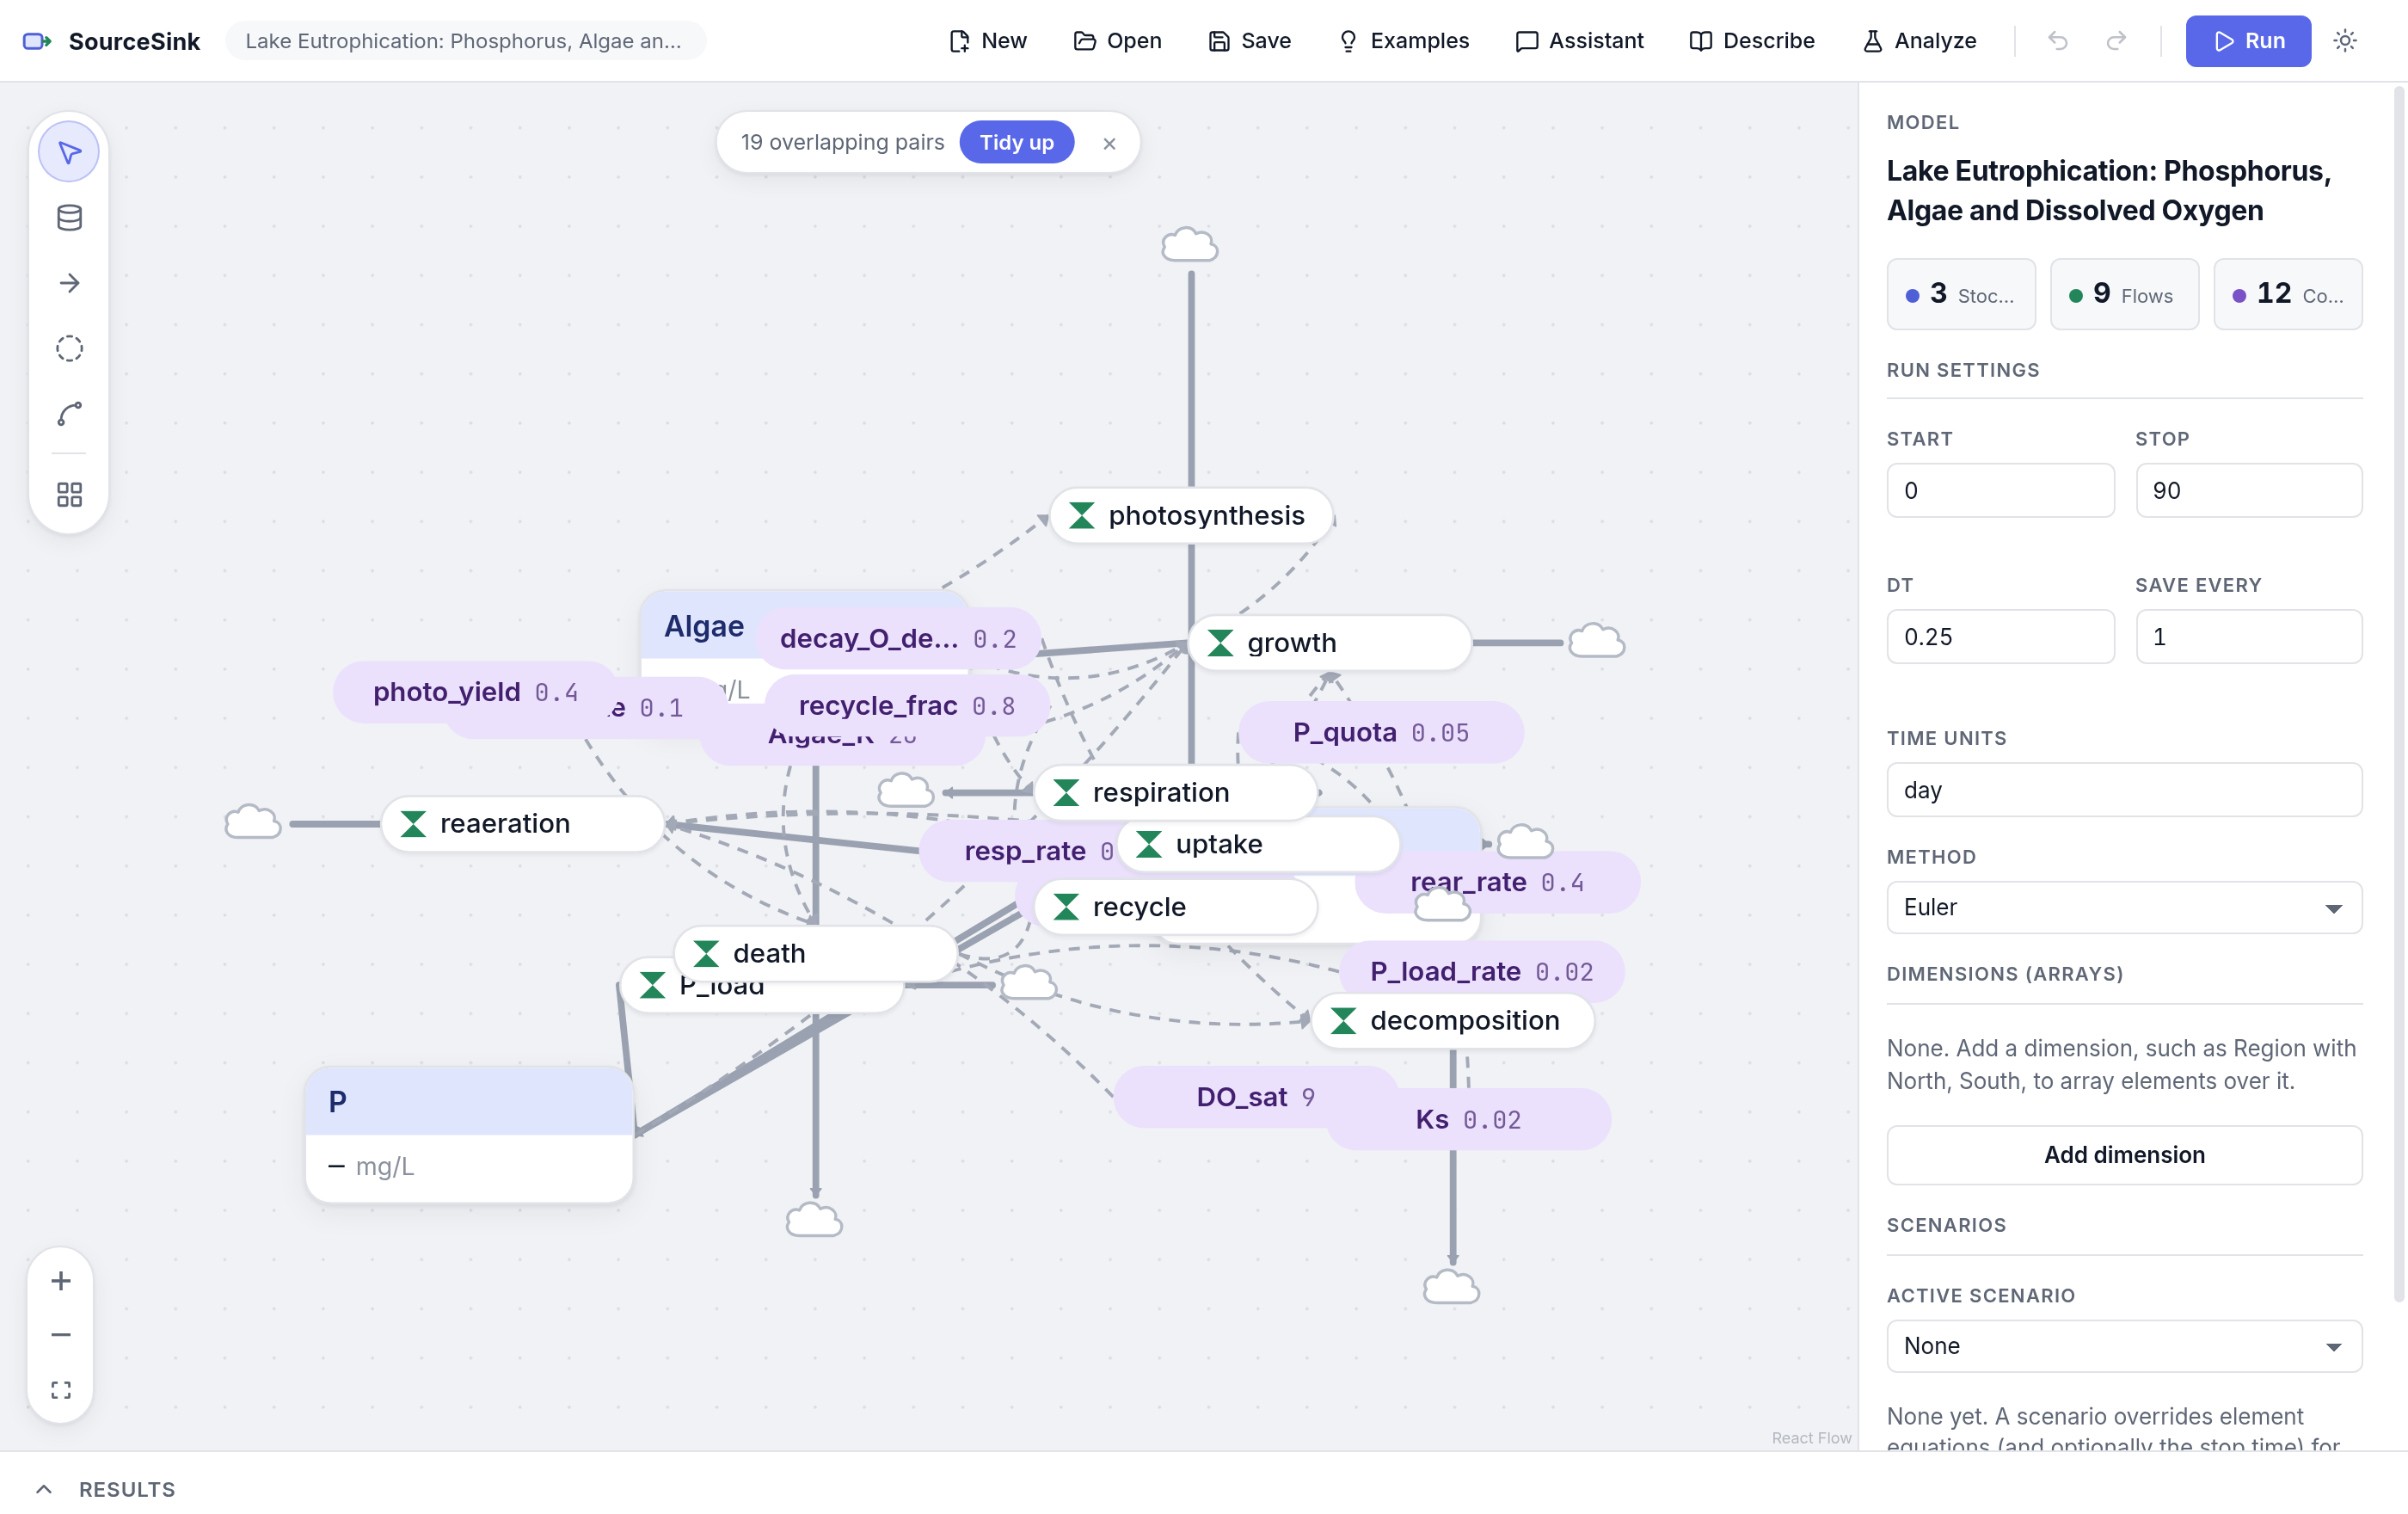
\includegraphics[width=0.8\textwidth]{img/tidy-before.png}\\[6pt]
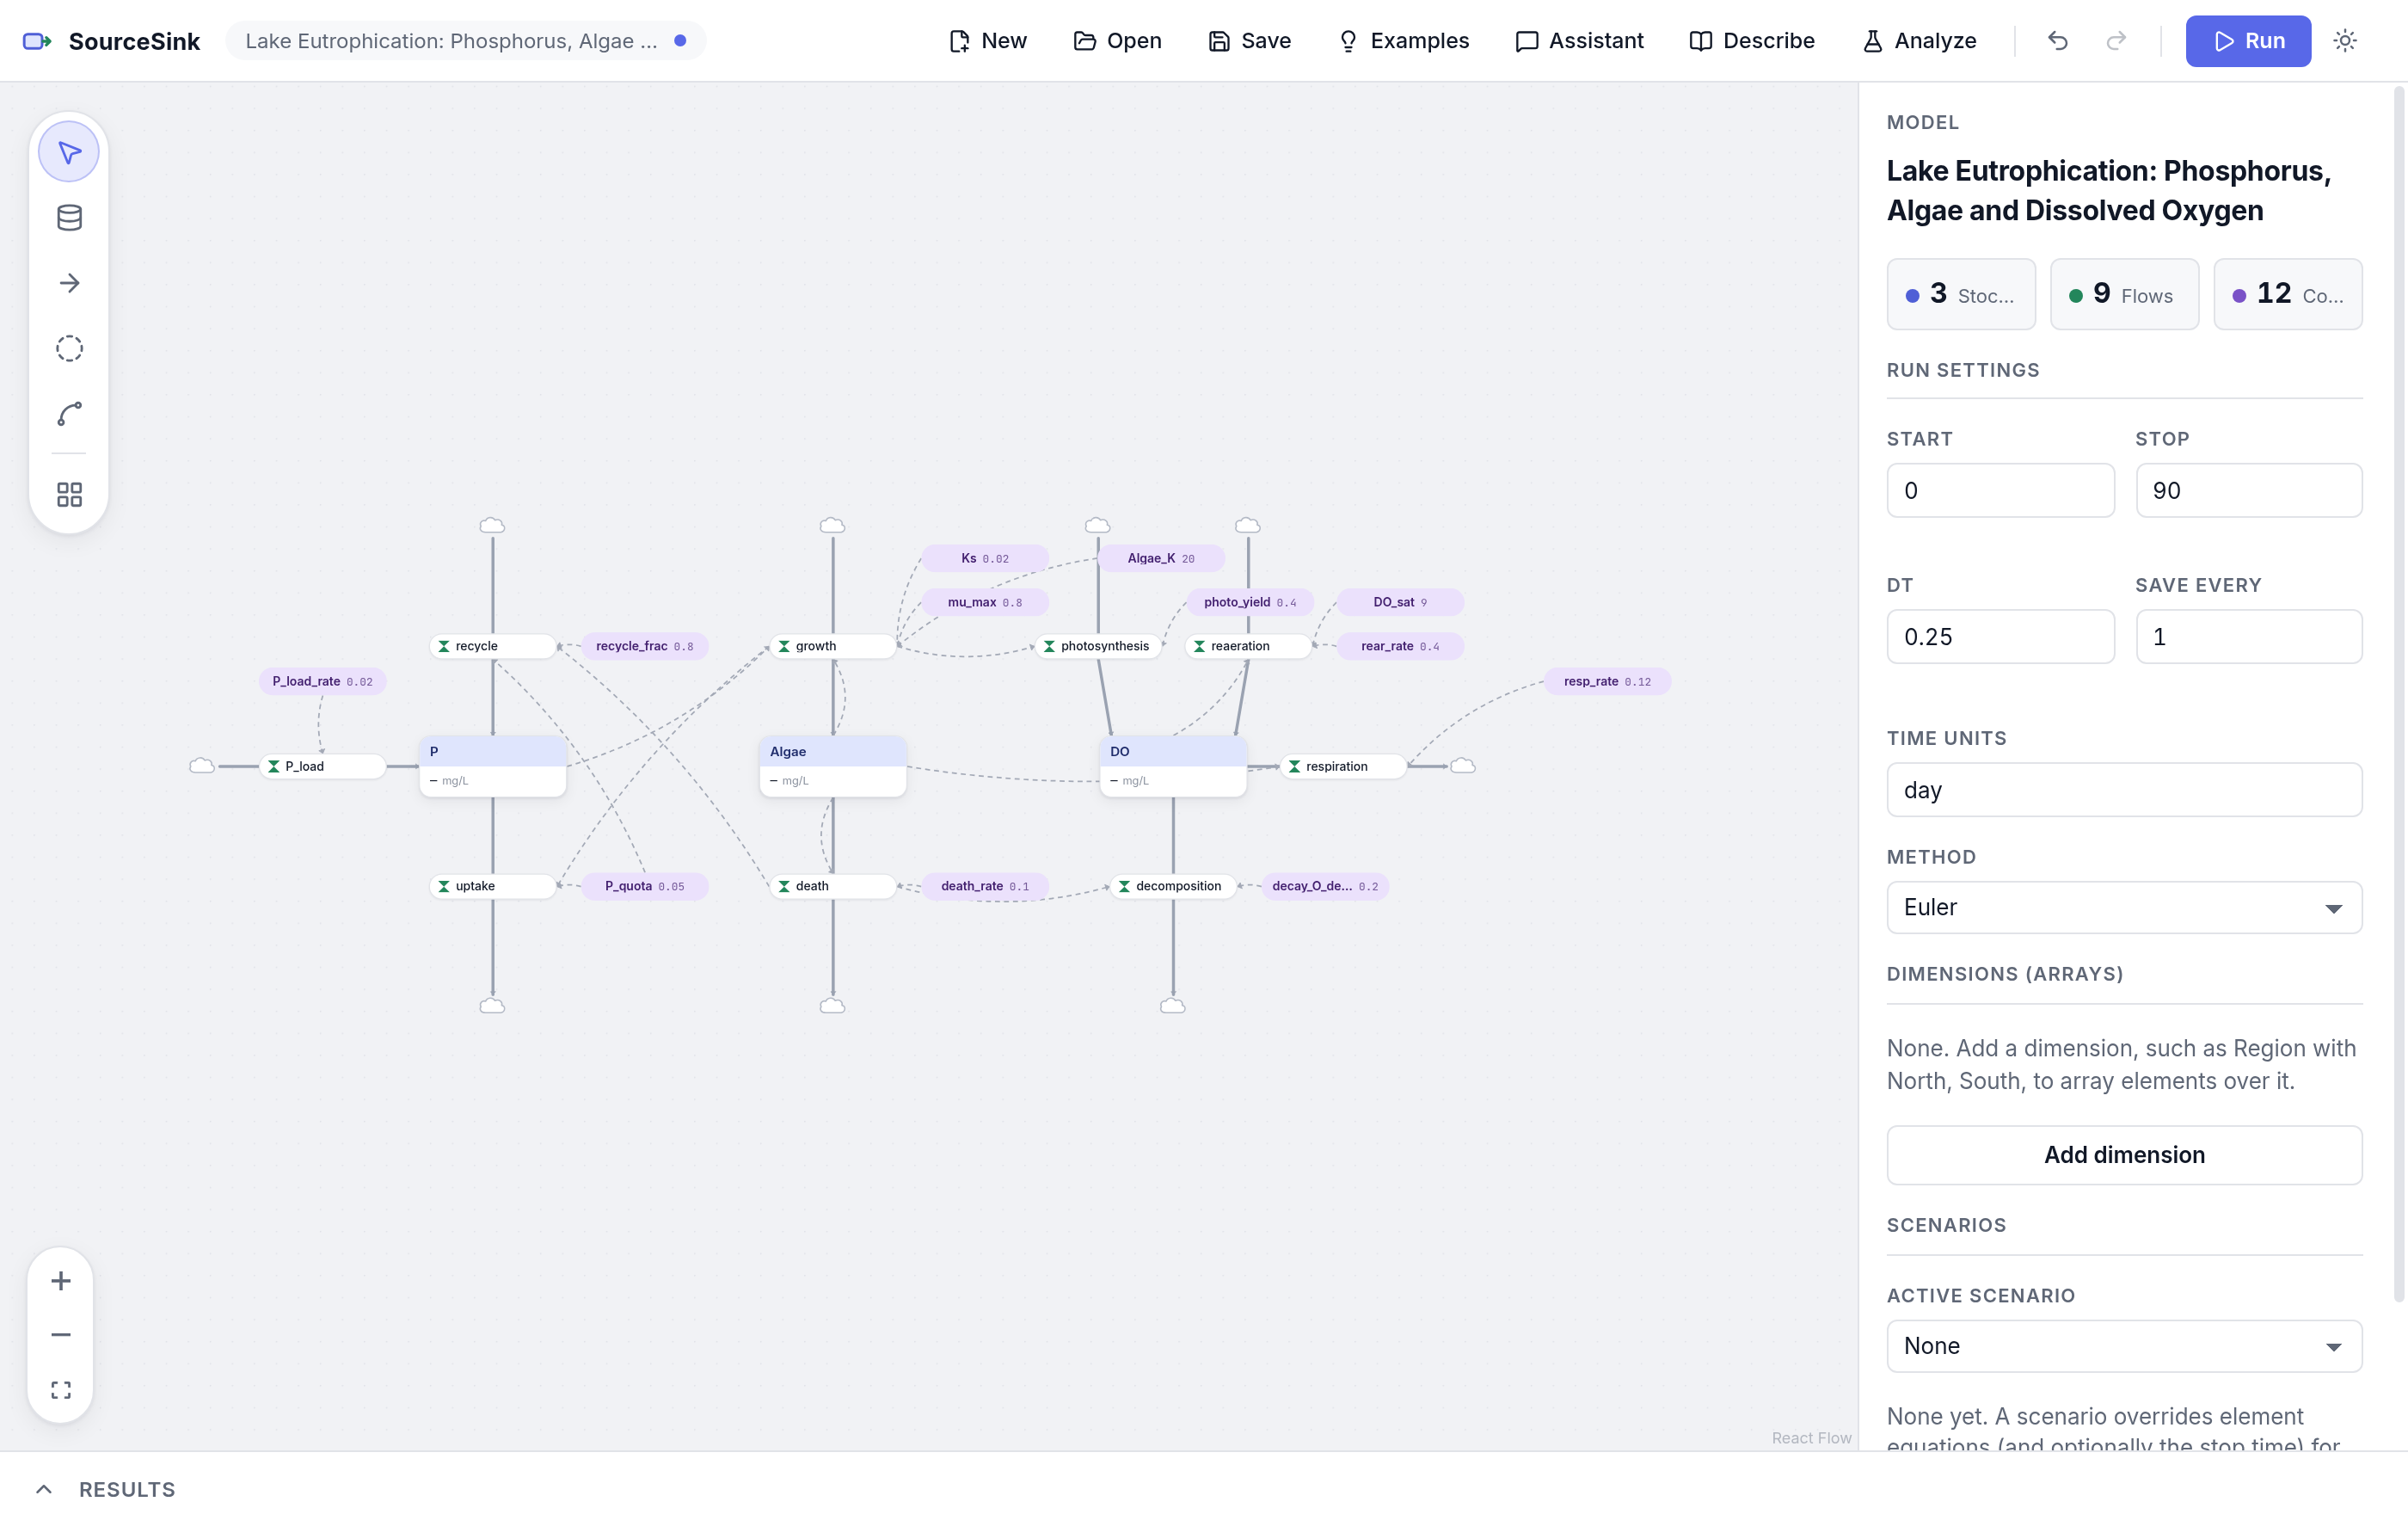
\includegraphics[width=0.8\textwidth]{img/tidy-after.png}
\caption{A lake eutrophication model before (top) and after (bottom) \ui{Tidy up}.}
\label{fig:tidy}
\end{figure}

The layout follows the usual conventions of stock-and-flow diagrams. Each
chain of stocks connected by flows gets its own row, ordered in the direction
material moves. Flows to and from the outside use the free ends of the row
first and then fan out above (inflows) or below (outflows) the stock. Flows
that run backwards, such as a recycle, loop below the row. Converters sit
next to the element they feed.

\section{Opening legacy models}

Click \ui{Open} and choose a \texttt{.stm} or \texttt{.itm} file. SourceSink
reads the model, its equations, graphical functions, arrays and diagram
positions, and reports in a notice anything it could not import faithfully. The original
arrangement is kept and spread out to suit SourceSink's larger shapes; use
\ui{Tidy up} if you prefer a fresh layout. Save the result as XMILE to keep
working with it.

% ================================================================ tutorial 7
\chapter{Tutorial 7: The command line}\label{ch:t7}

Everything you have done in the app can be scripted. The \texttt{sourcesink}
command runs models, sweeps parameters, fits data and runs sensitivity
analyses, and writes CSV or JSON for other tools. From a copy of the
repository, use \texttt{npx tsx src/cli/src/run.ts} in place of
\texttt{sourcesink}.

\begin{lstlisting}
# Run a model and print selected series as CSV
sourcesink run examples/environmental/streeter-phelps.xmile --columns BOD,DO

# Check units
sourcesink units examples/environmental/streeter-phelps.xmile

# Describe the model in plain language
sourcesink explain examples/environmental/streeter-phelps.xmile

# Monte Carlo with Latin hypercube sampling
sourcesink montecarlo examples/environmental/streeter-phelps.xmile \
  --param kd=0.2:0.5 --runs 200 --lhs --columns DO_deficit --percentiles 5,50,95

# Morris screening of the deficit peak
sourcesink sensitivity examples/environmental/streeter-phelps.xmile \
  --param kd=0.2:0.5 --param ka=0.4:0.8 --metric DO_deficit:max
\end{lstlisting}

The complete reference for every command and option, the model file format
and the MCP server (which lets AI agents build and analyze models through
SourceSink) is in \texttt{docs/llm/cli-guide.md}.

% ================================================================ reference
\chapter{Reference}\label{ch:ref}

\section{Elements and their options}

\paragraph{Stocks.} Equation = initial value. \ui{Non-negative} keeps the
stock at or above zero by limiting its outflows. A stock can also be a
\emph{conveyor} (material rides for a transit time, optionally with a
capacity and leakage), a \emph{queue} (first in, first out) or an
\emph{oven} (fills, cooks for a time, empties), the discrete-event stocks used
for queues, pipelines and batch processes.

\paragraph{Flows.} \ui{Uniflow} prevents negative values; \ui{Biflow} allows
the flow to run both ways. A flow out of a conveyor can be a \emph{leak}.

\paragraph{Converters.} A constant or an equation. A converter can also be a
graphical function: a lookup table of points with linear, held (step) or
discrete interpolation.

\paragraph{Arrays.} Under \ui{Dimensions} (nothing selected), define a
dimension such as \el{Region} with elements \el{North, South}. Any element
can then be arrayed over it, with one equation for all elements or one per
element.

\section{Integration methods}\label{sec:methods}

\begin{center}
\renewcommand{\arraystretch}{1.3}
\begin{tabularx}{\textwidth}{@{}l X@{}}
\toprule
\textbf{\sffamily Method} & \textbf{\sffamily Update for $\dot S = f(t, S)$ with step $h$}\\
\midrule
Euler & $S_{n+1} = S_n + h\,f(t_n, S_n)$. First order: error $\propto h$.\\
Runge--Kutta 2 (Heun) & $k_1 = f(t_n,S_n)$, $k_2 = f(t_n + h, S_n + h k_1)$, $S_{n+1} = S_n + \tfrac{h}{2}(k_1 + k_2)$.\\
Runge--Kutta 4 & $S_{n+1} = S_n + \tfrac{h}{6}(k_1 + 2k_2 + 2k_3 + k_4)$ with the classic four stages. Error $\propto h^{4}$.\\
Adaptive (RK45) & Dormand--Prince pair: estimates its own error each step and shrinks or grows the step to meet a tolerance. Best for stiff or fast models.\\
\bottomrule
\end{tabularx}
\end{center}

\section{Analysis methods at a glance}

\begin{center}
\renewcommand{\arraystretch}{1.25}
\begin{tabularx}{\textwidth}{@{}l l X@{}}
\toprule
\textbf{\sffamily Question} & \textbf{\sffamily Tool} & \textbf{\sffamily Output}\\
\midrule
What values fit my data? & Calibrate & Estimates $\pm$ standard errors, RMSE, NSE, $R^2$, bias, identifiability warnings\\
Which parameters matter? & Morris & $\mu^{*}$ (importance) and $\sigma$ (interaction) per parameter\\
How much of the variance? & Sobol & $S_1$ and $S_T$ with confidence intervals\\
How wide are the outcomes? & Uncertainty & Median and percentile bands over time\\
What if a value changes? & Scenarios & A separate run with overridden equations\\
\bottomrule
\end{tabularx}
\end{center}

\section{Themes}

The sun/moon button at the top right switches between light, dark and
``follow the system.'' Figure~\ref{fig:dark.png} shows the dark theme.

\shot{dark.png}{The dark theme with the lake eutrophication example after a run.}

% ================================================================ appendices
\appendix

\chapter{Equation functions}\label{app:functions}

Equations use $+$, $-$, $*$, $/$, \verb|^|, comparisons
(\verb|<|, \verb|<=|, \verb|>|, \verb|>=|, \verb|=|, \verb|<>|), \texttt{AND},
\texttt{OR}, \texttt{NOT} and \texttt{IF} \emph{condition} \texttt{THEN}
\emph{a} \texttt{ELSE} \emph{b}. \texttt{TIME} is the current time and
\texttt{DT} the time step. Names are case-insensitive.

\begingroup\small
\renewcommand{\arraystretch}{1.15}
\begin{longtable}{@{}>{\raggedright\ttfamily}p{0.40\textwidth} p{0.56\textwidth}@{}}
\toprule
\textrm{\textbf{\sffamily Function}} & \textbf{\sffamily Meaning}\\
\midrule
\endhead
\multicolumn{2}{@{}l}{\sffamily\bfseries\color{accent} Mathematics}\\
ABS(x), SQRT(x), EXP(x) & absolute value, square root, $e^{x}$\\
LN(x), LOG10(x) & natural and base-10 logarithm\\
SIN, COS, TAN, ARCTAN & trigonometry in radians\\
MIN(a,b,…), MAX(a,b,…) & smallest and largest argument\\
MOD(a,b), INT(x), ROUND(x) & remainder, floor ($\mathrm{INT}(-8.9) = -9$), nearest integer\\
POWER(a,b) & $a^{b}$\\
SUM, MEAN, STDDEV & sum, mean and population standard deviation of the arguments\\
\multicolumn{2}{@{}l}{\sffamily\bfseries\color{accent} Time inputs}\\
STEP(h, t) & 0 before time $t$, $h$ from $t$ on\\
RAMP(slope, start, end) & rises at \emph{slope} from \emph{start} until \emph{end}\\
PULSE(v, first, interval) & moves volume $v$ in one DT, repeating every \emph{interval}\\
SINWAVE(a, p), COSWAVE(a, p) & periodic inputs of amplitude $a$ and period $p$\\
\multicolumn{2}{@{}l}{\sffamily\bfseries\color{accent} Delays and smoothing}\\
DELAY1(in, d), DELAY3(in, d) & first- and third-order material delays\\
DELAYN(in, d, init, n) & $n$th-order material delay\\
DELAY(in, d) & pipeline delay: the input as it was $d$ time units ago\\
SMTH1(in, t), SMTH3(in, t), SMTHN(in, t, n) & exponential smoothing (first, third, $n$th order)\\
TREND(in, t), FORCST(in, t, h) & fractional trend; extrapolation $h$ time units ahead\\
\multicolumn{2}{@{}l}{\sffamily\bfseries\color{accent} Random numbers (repeatable with a seed)}\\
RANDOM(min, max), NORMAL(m, s) & uniform and normal random values\\
EXPRND(mean), POISSON(mu) & exponential and Poisson random values\\
MONTECARLO(p) & 1 with probability $p$\% per time unit\\
\multicolumn{2}{@{}l}{\sffamily\bfseries\color{accent} Finance}\\
PV, FV, PMT, NPV & present value, future value, payment, net present value\\
CGROWTH(pct) & DT-independent compound growth rate\\
\multicolumn{2}{@{}l}{\sffamily\bfseries\color{accent} Discrete stocks and cycle times}\\
QLEN, QELEM, CAP & queue length, element of a queue or conveyor, capacity\\
TRANSTIME, COOKTIME, OSTATE & conveyor transit time, oven cook time and state\\
CTMEAN, CTMIN, CTMAX, CTSTDDEV, CYCLETIME, THROUGHPUT & cycle-time statistics\\
\multicolumn{2}{@{}l}{\sffamily\bfseries\color{accent} Other}\\
PREVIOUS(x), INIT(x) & value one DT ago; value at the start\\
COUNTER(a, b), SWITCH(a, b), PCT(x) & counter; $1$ if $a>b$; $100x$\\
DERIVN(x, n) & $n$th time derivative by backward differences\\
\bottomrule
\end{longtable}
\endgroup

\chapter{Units}\label{app:units}

Write units the way you would on paper:
\texttt{mg/L}, \texttt{1/day}, \texttt{m3/s} (a digit after a letter is an
exponent), \texttt{m\^{}3}, \texttt{kg m-2}, \texttt{tonnes/year},
\texttt{people}, \texttt{\%}, \texttt{dimensionless}. Time units are
recognized in their common forms (s, min, h, day, week, month, year) and
convert to one another; masses (mg, g, kg, tonne), lengths (mm, cm, m, km) and
volumes (mL, L, m3) also convert. Any other word, such as \texttt{fish} or
\texttt{dollars}, is its own unit.

\chapter{Keyboard shortcuts}\label{app:keys}

\begin{center}
\renewcommand{\arraystretch}{1.3}
\begin{tabular}{@{}l l@{\hspace{3em}}l l@{}}
\toprule
\key{V} & Select tool & \key{Ctrl}+\key{S} & Save\\
\key{S} & Stock tool & \key{Ctrl}+\key{Shift}+\key{S} & Save as\\
\key{F} & Flow tool & \key{Ctrl}+\key{O} & Open\\
\key{C} & Converter tool & \key{Ctrl}+\key{Z} & Undo\\
\key{K} & Connector tool & \key{Ctrl}+\key{Y} & Redo\\
\key{L} & Tidy up the layout & \key{Ctrl}+\key{Enter} & Run\\
\key{Esc} & Select tool, clear selection & \key{Delete} & Delete the selection\\
\bottomrule
\end{tabular}
\end{center}

\chapter{Troubleshooting}\label{app:trouble}

\begin{description}[style=nextline,leftmargin=1.2em,font=\sffamily\bfseries\color{ink}]
\item[A stock shoots to enormous values or NaN.] The model is probably stiff
for the chosen DT. Halve DT, or choose \ui{Adaptive (RK45)}. Check that a
rate is not in the wrong time units (a unit warning usually says so).
\item[A stock goes negative and should not.] Tick \ui{Non-negative} on the
stock, or make the outflow depend on the stock so it shrinks as the stock
empties.
\item[An equation says a name is unknown.] Check the spelling, and connect
the element with the connector tool (\key{K}); the inspector offers to add
the missing connector.
\item[Calibration does not converge.] Narrow the parameter ranges, use
\ui{log} for parameters spanning orders of magnitude, add restarts, or try
differential evolution. Read the identifiability warnings: two parameters
that always move together cannot both be estimated from these data.
\item[The assistant is unavailable.] Install OpenCode, run
\texttt{opencode providers} to sign in to OpenRouter, then click
\ui{Check again} in the panel.
\end{description}

% ================================================================ references
\begin{thebibliography}{99}\small
\addcontentsline{toc}{chapter}{References}
\bibitem{bass1969} Bass, F.~M. (1969). A new product growth for model consumer durables. \emph{Management Science}, 15(5), 215--227. \url{https://doi.org/10.1287/mnsc.15.5.215}
\bibitem{harte1988} Harte, J. (1988). \emph{Consider a Spherical Cow: A Course in Environmental Problem Solving}. University Science Books.
\bibitem{morris1991} Morris, M.~D. (1991). Factorial sampling plans for preliminary computational experiments. \emph{Technometrics}, 33(2), 161--174. \url{https://doi.org/10.1080/00401706.1991.10484804}
\bibitem{saltelli2010} Saltelli, A., Annoni, P., Azzini, I., Campolongo, F., Ratto, M., \& Tarantola, S. (2010). Variance based sensitivity analysis of model output. Design and estimator for the total sensitivity index. \emph{Computer Physics Communications}, 181(2), 259--270. \url{https://doi.org/10.1016/j.cpc.2009.09.018}
\bibitem{streeter1925} Streeter, H.~W., \& Phelps, E.~B. (1925). A study of the pollution and natural purification of the Ohio River. III. Factors concerned in the phenomena of oxidation and reaeration. Public Health Bulletin No.~146, U.S. Public Health Service.
\bibitem{vollenweider1975} Vollenweider, R.~A. (1975). Input-output models with special reference to the phosphorus loading concept in limnology. \emph{Schweizerische Zeitschrift für Hydrologie}, 37(1), 53--84. \url{https://doi.org/10.1007/BF02505178}
\end{thebibliography}

\end{document}
